\newcommand{\streamlinecomment}[1]{}


\begin{ccTexOnly}
\begin{center}
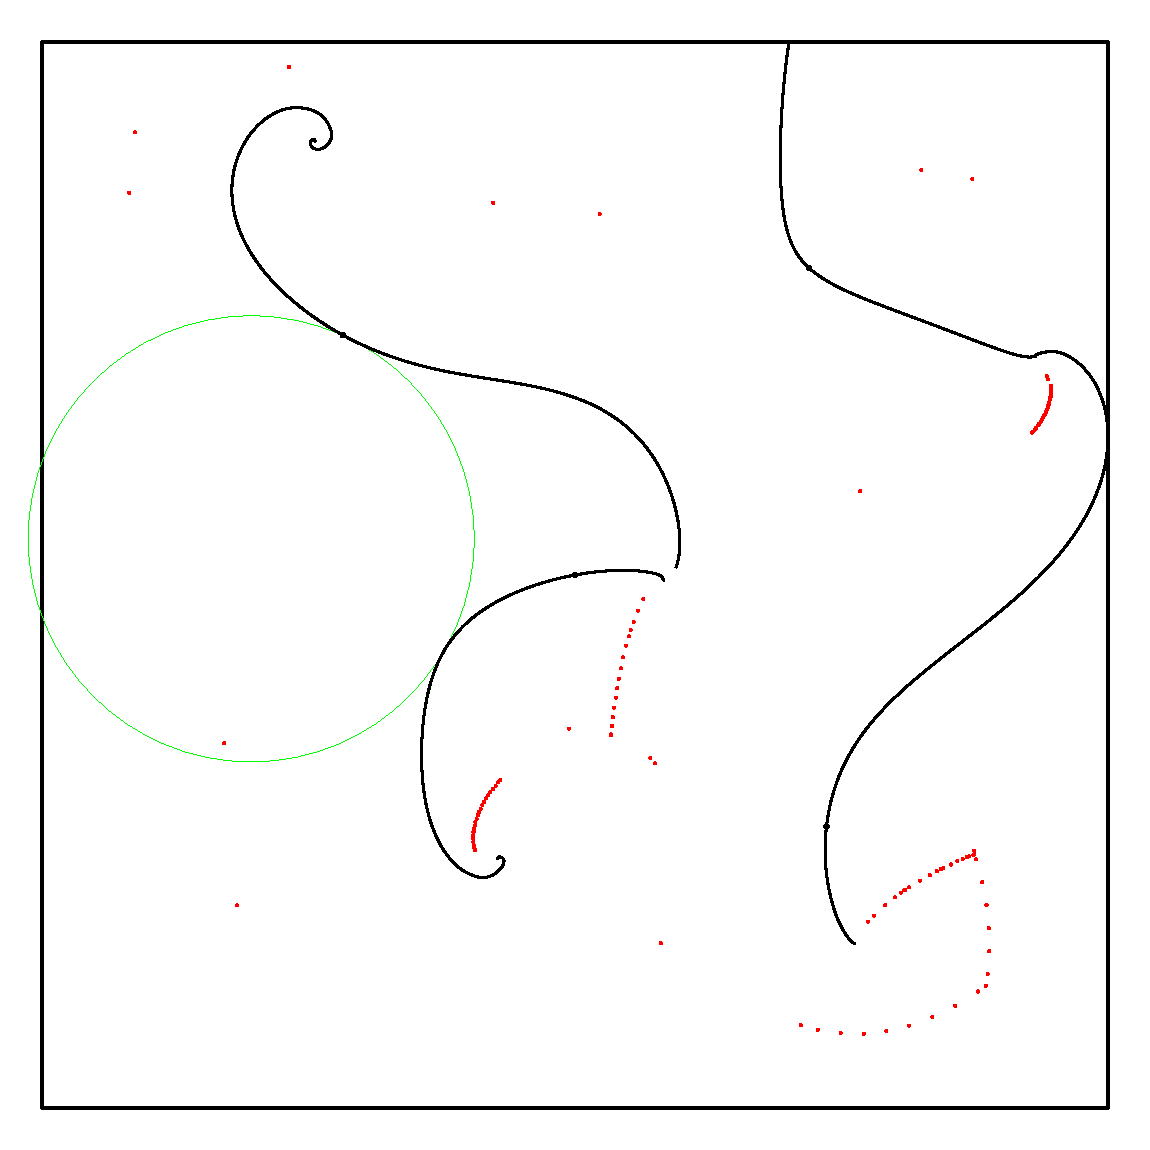
\includegraphics[width=4cm]{Stream_lines_2/1} \hspace*{0.5cm} 
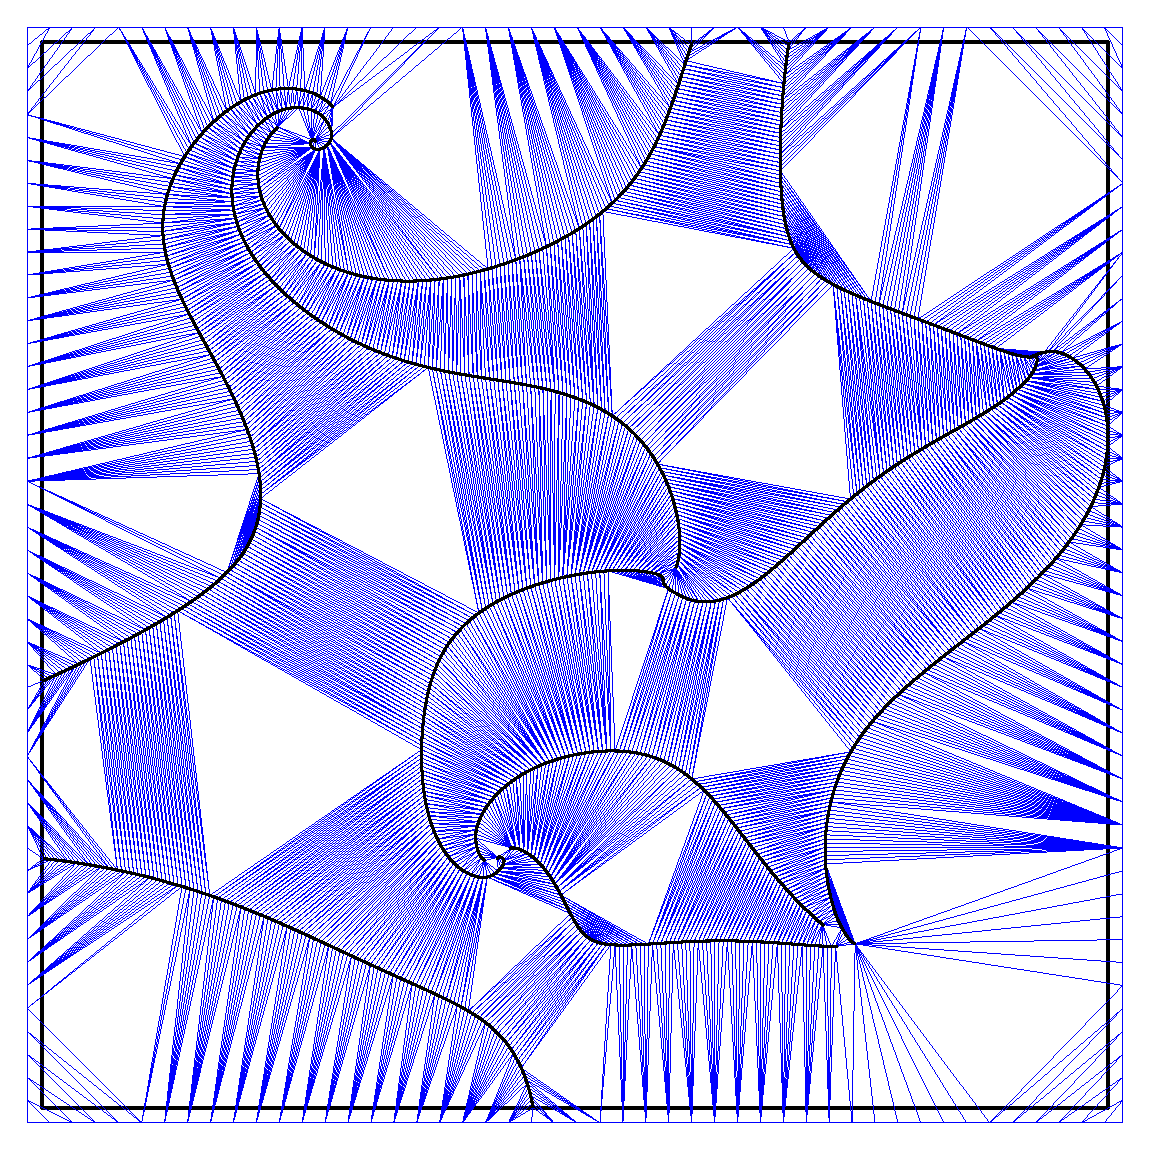
\includegraphics[width=4cm]{Stream_lines_2/2} \hspace*{0.5cm} 
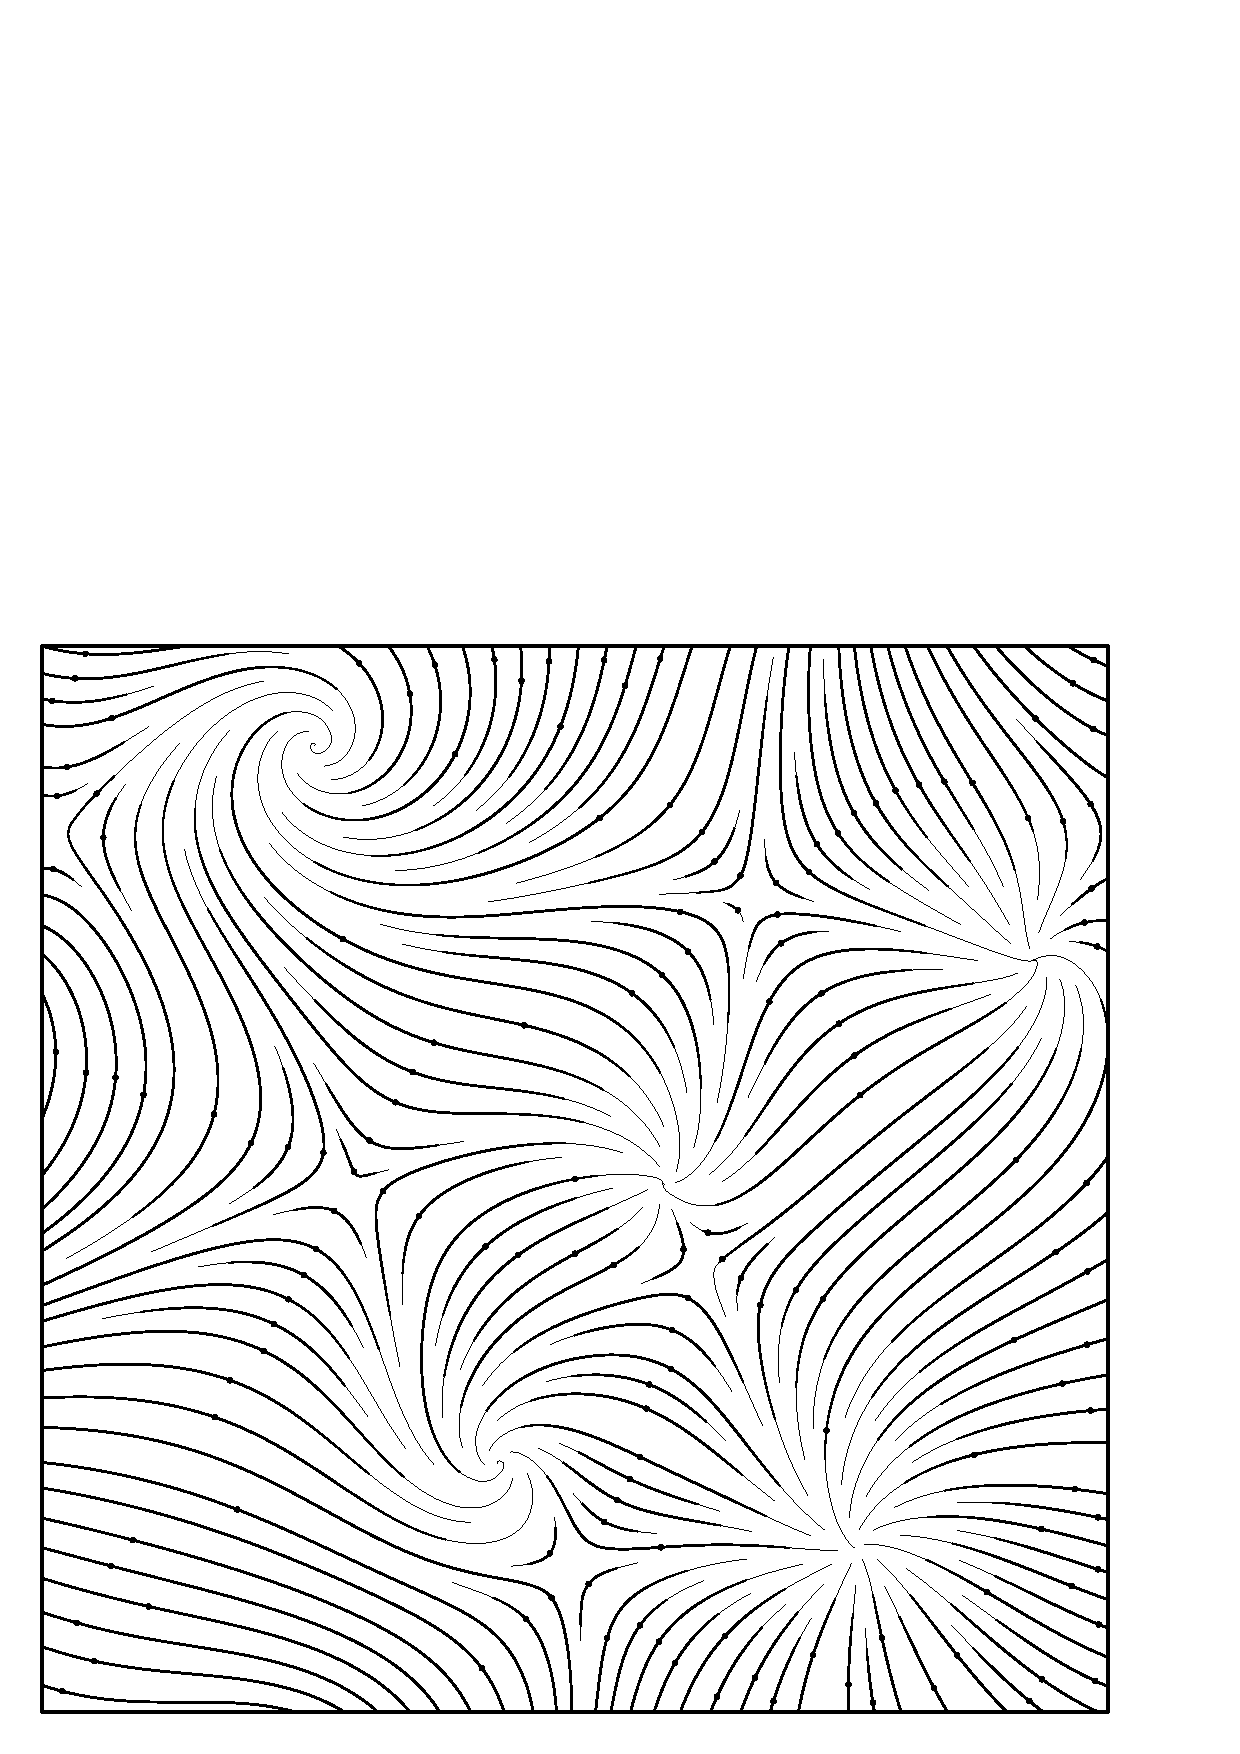
\includegraphics[width=4cm]{Stream_lines_2/3} 
\end{center}
\end{ccTexOnly}

% \begin{ccHtmlOnly}
% <CENTER>
% <img border=0 src="./tr1.gif" width=300>
% <img border=0 src="./dt1.gif" width=300>
% </CENTER>
% \end{ccHtmlOnly}

This chapter describes the \cgal's 2D streamline placement package.
Basic definitions and notions are given in section
\ref{Section_2D_Streamlines_Definitions}. Section
\ref{Section_2D_Streamlines_Strategy} describes briefly the algorithm. Section
\ref{Section_2D_Streamlines_Implementation} presents the implementation of the package. Section
\ref{Section_2D_Streamlines_Example} gives two examples of using the package.

\section{Definitions}
\label{Section_2D_Streamlines_Definitions}
Vector and direction fields are commonly used for modeling physical
phenomena, where a direction and magnitude, or a vector is assigned to
each point inside a domain. Streamlines are very important tools for
visualizing those entites. A \ccc{streamline} is a curve
everywhere tangent to the field.  A streamline can be considered as
the path traced by an imaginary massless particle dropped into a
steady fluid flow described by the field. In practice, a streamline is
often represented as a polyline iteratively elongated by bidirectional
numerical integration started from a \ccc{seed point}, until it comes
close to another streamline, hits the domain boundary, reaches a
critical point or generates a closed path. A \ccc{valid} placement of
streamlines consists of saturating the domain with a set of tangential
streamlines in accordance with a specified density.

\section{Farthest point seeding streategy}
\label{Section_2D_Streamlines_Strategy}
The algorithm implemented in this package (add reference) consists of placing
one streamline at a time by numerical integration starting at the furthest away
from all previously placed streamlines.\\The input of our algorithm is given by
(i) a flow field, (ii) a \textit{density} specified either globally by the
inverse of the ideal spacing distance, or locally by a density field, and (iii)
a \textit{saturation} ratio over the desired spacing required to trigger the
seeding of a new streamline.\\The input flow field is given by a discrete set of
vectors or directions sampled within a domain, associated with an interpolation
scheme (\textit{e.g.} bilinear interpolation over a regular grid, or natural
neighbor interpolation over an irregular point set to
allow for an evaluation at each point coordinate within the domain).\\The
\textit{output} is a streamline placement, represented as a list of streamlines.
The core idea of our algorithm consists of placing one streamline at a time by
numerical integration seeded at the farthest point from all previously placed
streamlines.\\The streamlines are approximated by polylines, whose points are
inserted in a 2D Delaunay triangulation. The empty circumscribed circles of the
Delaunay triangles provide us with a good approximation of the cavities in the
domain.\\After each streamline integration, all incident triangles which
circumcircle diameter is larger (within the saturation ratio) than the desired
spacing distance are pushed to a priority queue sorted by the triangle
circumcircle diameter. To start each new streamline integration, the triangle
with largest circumcircle diameter (and hence the biggest cavity) is popped out
of the queue. We first test if it is still a valid triangle of the
triangulation, since it could have been destroyed by a streamline previously
added to the triangulation. If not, we pop another triangle out of the queue. If
yes, we use the center of its circumcircle as seed point to integrate a new
streamline.\\Our algorithm terminates when the priority queue is empty. The size
of the biggest cavity being monotonically decreasing, our algorithm guarantees
the domain saturation.

\subsection{Implementation}
\label{Section_2D_Streamlines_Implementation}
Streamlines are represented as polylines, and are obtained by iteraive
integration form the seed point. The computation is processed via a list of
Delaunay triangulation vertices.\\To implement the triangular grid, the CGAL 2D
Delaunay triangulation is used. The priority queue used to store candidate seed
points is taken from the Standard Template Library~\cite{cgal:sgcsi-stlpg-97}.

\section{Example}
\label{Section_2D_Streamlines_Example}
The first example illustrates the generation of a 2D streamline placement from a 
vector field defined on a regular grid.
\ccIncludeExampleCode{Stream_lines_2/stl_regular_field.C}
The second example depicts the generation of a streamline placement from a vector
field defined on a triangular grid.
\ccIncludeExampleCode{Stream_lines_2/stl_triangular_field.C}
